% Options for packages loaded elsewhere
\PassOptionsToPackage{unicode}{hyperref}
\PassOptionsToPackage{hyphens}{url}
%
\documentclass[
]{article}
\usepackage{lmodern}
\usepackage{amssymb,amsmath}
\usepackage{ifxetex,ifluatex}
\ifnum 0\ifxetex 1\fi\ifluatex 1\fi=0 % if pdftex
  \usepackage[T1]{fontenc}
  \usepackage[utf8]{inputenc}
  \usepackage{textcomp} % provide euro and other symbols
\else % if luatex or xetex
  \usepackage{unicode-math}
  \defaultfontfeatures{Scale=MatchLowercase}
  \defaultfontfeatures[\rmfamily]{Ligatures=TeX,Scale=1}
\fi
% Use upquote if available, for straight quotes in verbatim environments
\IfFileExists{upquote.sty}{\usepackage{upquote}}{}
\IfFileExists{microtype.sty}{% use microtype if available
  \usepackage[]{microtype}
  \UseMicrotypeSet[protrusion]{basicmath} % disable protrusion for tt fonts
}{}
\makeatletter
\@ifundefined{KOMAClassName}{% if non-KOMA class
  \IfFileExists{parskip.sty}{%
    \usepackage{parskip}
  }{% else
    \setlength{\parindent}{0pt}
    \setlength{\parskip}{6pt plus 2pt minus 1pt}}
}{% if KOMA class
  \KOMAoptions{parskip=half}}
\makeatother
\usepackage{xcolor}
\IfFileExists{xurl.sty}{\usepackage{xurl}}{} % add URL line breaks if available
\IfFileExists{bookmark.sty}{\usepackage{bookmark}}{\usepackage{hyperref}}
\hypersetup{
  pdftitle={Propuesta de mejora de proceso de gestión de inventario, mediante la implementación de WMS para el caso de área de almacén del taller de servicio mecánico integral y electricidad automotriz DUARCON},
  pdfauthor={Felipe Kiefer Guenupan},
  hidelinks,
  pdfcreator={LaTeX via pandoc}}
\urlstyle{same} % disable monospaced font for URLs
\usepackage[margin=1in]{geometry}
\usepackage{graphicx}
\makeatletter
\def\maxwidth{\ifdim\Gin@nat@width>\linewidth\linewidth\else\Gin@nat@width\fi}
\def\maxheight{\ifdim\Gin@nat@height>\textheight\textheight\else\Gin@nat@height\fi}
\makeatother
% Scale images if necessary, so that they will not overflow the page
% margins by default, and it is still possible to overwrite the defaults
% using explicit options in \includegraphics[width, height, ...]{}
\setkeys{Gin}{width=\maxwidth,height=\maxheight,keepaspectratio}
% Set default figure placement to htbp
\makeatletter
\def\fps@figure{htbp}
\makeatother
\setlength{\emergencystretch}{3em} % prevent overfull lines
\providecommand{\tightlist}{%
  \setlength{\itemsep}{0pt}\setlength{\parskip}{0pt}}
\setcounter{secnumdepth}{-\maxdimen} % remove section numbering

\title{Propuesta de mejora de proceso de gestión de inventario, mediante
la implementación de WMS para el caso de área de almacén del taller de
servicio mecánico integral y electricidad automotriz DUARCON}
\usepackage{etoolbox}
\makeatletter
\providecommand{\subtitle}[1]{% add subtitle to \maketitle
  \apptocmd{\@title}{\par {\large #1 \par}}{}{}
}
\makeatother
\subtitle{Trabajo de titulación presentado en conformidad a los
requisitos para obtener el Titulo de Ingueniero Civil Industrial TESIS
PARA TITULO PARA LA OBTENCIÓN DEL TITULO INGENIERO CIVIL INDUSTRIAL}
\author{Felipe Kiefer Guenupan}
\date{\today}

\begin{document}
\maketitle

\newpage

\newpage

\hypertarget{introducciuxf3n}{%
\section{Introducción}\label{introducciuxf3n}}

\hypertarget{antecedentes-situaciuxf3n-actual-mercado-automuxf3vil}{%
\subsection{Antecedentes, situación actual mercado
automóvil}\label{antecedentes-situaciuxf3n-actual-mercado-automuxf3vil}}

El inicio de la pandemia del COVID-19 a afectado la venta de automóvil,
el primer semestre del año 2020 hubo una reducción en la compra de
vehículos livianos y medianos. la figura @ref(fig:vauto) presenta las
ventas del mercado automotor de livianos y medianos, realizado por
Asociación Nacional Automotriz de Chile (ANAC).

\begin{figure}
\centering
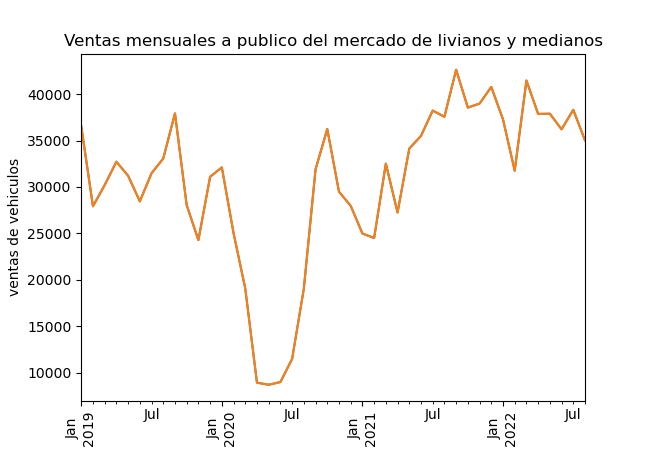
\includegraphics{fig/anac.png}
\caption{anac}
\end{figure}

En primera instancia en el gráfico se puede observar un valle debido a
``principalmente, por el deterioro de las condiciones económicas a nivel
internacional que han afectado a distintos mercados, no solo el
automotriz, las cuales se han visto acrecentadas por las circunstancias
políticas y económicas a nivel local''\footnote{ANAC Informe Mercado
  Automotor Febrero 2020}, posterior debido al desconfinamiento
progresivo a nivel nacional de ciertas comunas por la implementación del
programa Paso a Paso, Adicionalmente, el factor del retiro del 10\% de
las AFP ha demostrado un nivel de incidencia certero en la adquisición
de bienes durables como los automóviles, lo que se sumaría a la
recuperación del sector \footnote{ANAC Informe Mercado Automotor
  Septiembre 2020}. Meses posteriores este mercado automotriz a visto
una disminucion en la variacion de ventas conrespecto al año movil. En
consecuencia se espera un aumento en la demanda de los servicios de
mantenimiento y reparación automotriz.

\hypertarget{descripciuxf3n-general-de-la-organizicion}{%
\subsection{Descripción general de la
organizicion}\label{descripciuxf3n-general-de-la-organizicion}}

Duarcon LTDA. es una pequeña empresa\footnote{\url{https://www.economia.gob.cl/wp-content/uploads/2014/04/Boletin-Revision-Clasificacion-Estatuto-Pyme.pdf}
  2021-11-08 20:53:40} dedicada la reparación mecánica y eléctrica
automotriz de vehículos livianos\footnote{Según definición ANAC},
ubicada en Lo Ovalle N 220, Quilicura, cuenta con una plantilla de 6
trabajadores (1 administrador y 5 mecánicos, detallado en la figura
@ref(fig:estruc)). Creada en el ano 2005, ha entregado sus servicios a
la comunidad cercana, su demanda constante del servicio impulso expandir
la plaza de servicio, desde 1000 ft\textsuperscript{2} a 2442
ft\textsuperscript{2}. Debido a la demanda del servicio el año 2009,
Duarcon LTDA. a incorpora a su taller un almacén con un área de 418, con
el propósito de alojar repuestos necesarios en el servicio de
reparación, en el segundo semestre del presente ano Duarcon LTDA., con
el fin agregar a su linea de negocio la venta de neumáticos se construye
otro almacén con un área de 243 ft\textsuperscript{2}, lo que da un
total de 661 ft\textsuperscript{2} de plaza para almacén (vease
@ref(fig:layout)).

\hypertarget{descripciuxf3n-de-la-organizaciuxf3n-historia-productos-y-mercados-principales-estructura-organizacional-tamauxf1o-etc.-quiuxe9n-soy}{%
\subsubsection{Descripción de la organización: historia, productos y
mercados principales, estructura organizacional, tamaño, etc. (¿Quién
soy?)}\label{descripciuxf3n-de-la-organizaciuxf3n-historia-productos-y-mercados-principales-estructura-organizacional-tamauxf1o-etc.-quiuxe9n-soy}}

Iniciada en 2005 entregaba el servicio de reparación electrica
complementario a un taller a vecino posterior incursiono en servicio de
mantencion para finalmente entregar servicio de mecanico integral a
perdurado en rubro de la reparación automotriz brindado a la comuna de
Quilicura el servicio de reparación electica

\hypertarget{descripciuxf3n-del-medio-en-el-cual-se-encuentra-la-organizaciuxf3n-caracteruxedsticas-de-la-industria-de-la-economuxeda-etc.-duxf3nde-estoy}{%
\subsubsection{Descripción del medio en el cual se encuentra la
organización: características de la industria, de la economía, etc.
(¿Dónde
estoy?)}\label{descripciuxf3n-del-medio-en-el-cual-se-encuentra-la-organizaciuxf3n-caracteruxedsticas-de-la-industria-de-la-economuxeda-etc.-duxf3nde-estoy}}

FODA

Fortalezas entrega de nuevos servicios

Oportunidades definir procesos

Debilidades estandarizar prestación Amenazas competencia

\hypertarget{servicios-que-brinda}{%
\subsubsection{Servicios que brinda}\label{servicios-que-brinda}}

La empresa brinda servicios automotrices tanto en el aspecto mecánico,
electrónico y de latonería. A continuación se desglosan todos los
servicios que se ofrecen.

Aspecto mecánico automotriz liviano-mediano.

\begin{itemize}
\tightlist
\item
  ABC de Motor.
\item
  VABC de Frenos.
\item
  Suspensión.
\end{itemize}

Embrague. Reparación de motores. Mantenimiento
Predictivo/Preventivo/Correctivo. Cambios de aceite al instante. Cambios
de Filtros de aire. Cambios de Filtros de polen. Reparación de cajas
automáticas con garantía. Reparación del sistema eléctrico del vehículo.
Controles de calidad. Limpieza de inyectores. Limpieza por ultrasonido.
Laboratorio de comprobación de inyectores. Filtros y o'rings de inyector
(Comercialización).

Diagnóstico computarizado. Diagnóstico para toda marca de vehículos.
Escáneres actualizados al 2010 (SPC, OTC). Frenos ABS. Sistema de
Airbag. OBD II.

\hypertarget{descripciuxf3n-de-la-estrategia-para-saber-cuuxe1l-es-la-direcciuxf3n-en-que-camina-la-empresa.-quuxe9-quiero}{%
\subsubsection{Descripción de la estrategia, para saber cuál es la
dirección en que camina la empresa. (¿Qué
quiero?)}\label{descripciuxf3n-de-la-estrategia-para-saber-cuuxe1l-es-la-direcciuxf3n-en-que-camina-la-empresa.-quuxe9-quiero}}

\hypertarget{descripciuxf3n-del-uxe1mbito-de-trabajo-propuxf3sito-personas-procesos-estructura-tecnologuxeda-etc.}{%
\subsubsection{Descripción del ámbito de trabajo: propósito, personas,
procesos, estructura, tecnología,
etc.}\label{descripciuxf3n-del-uxe1mbito-de-trabajo-propuxf3sito-personas-procesos-estructura-tecnologuxeda-etc.}}

El lugar de trabajo esta clasificado en área de servicio, area de
almacen, area compresor, servicio higene, casino.

\begin{figure}
\centering
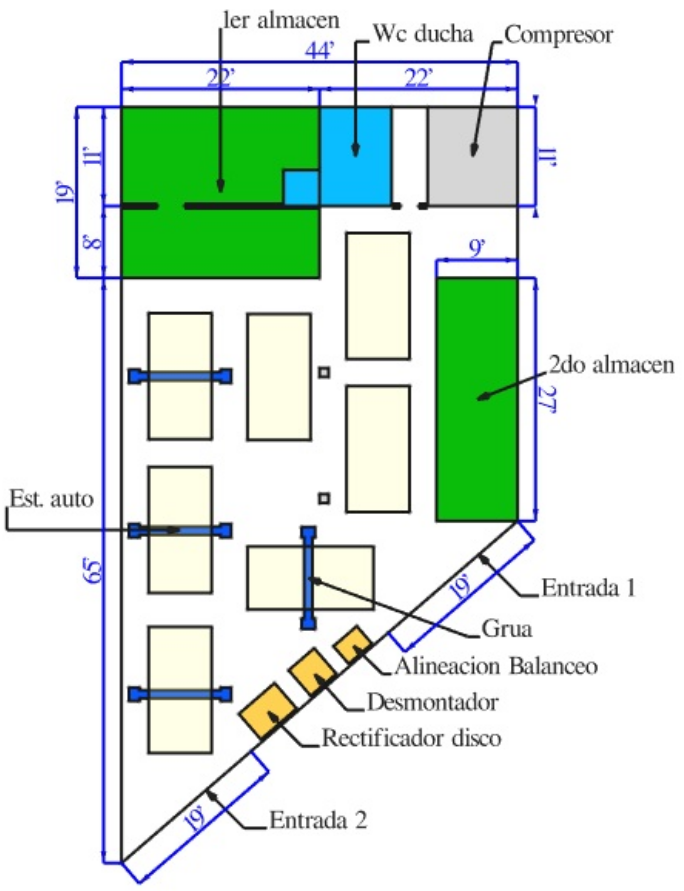
\includegraphics{fig/plan.png}
\caption{plan}
\end{figure}

\hypertarget{descripciuxf3n-del-entorno-inmediato-y-relaciones-ubicaciuxf3n-del-uxe1mbito-de-trabajo-relaciones-con-otras-uxe1reas-quuxe9-y-a-quiuxe9nes-provee-de-quiuxe9nes-recibe-quuxe9-etc.}{%
\subsubsection{Descripción del entorno inmediato y relaciones: ubicación
del ámbito de trabajo: relaciones con otras áreas, qué y a quiénes
provee, de quiénes recibe qué,
etc.}\label{descripciuxf3n-del-entorno-inmediato-y-relaciones-ubicaciuxf3n-del-uxe1mbito-de-trabajo-relaciones-con-otras-uxe1reas-quuxe9-y-a-quiuxe9nes-provee-de-quiuxe9nes-recibe-quuxe9-etc.}}

Duarcon LTDA. proveedores

\begin{figure}
\centering
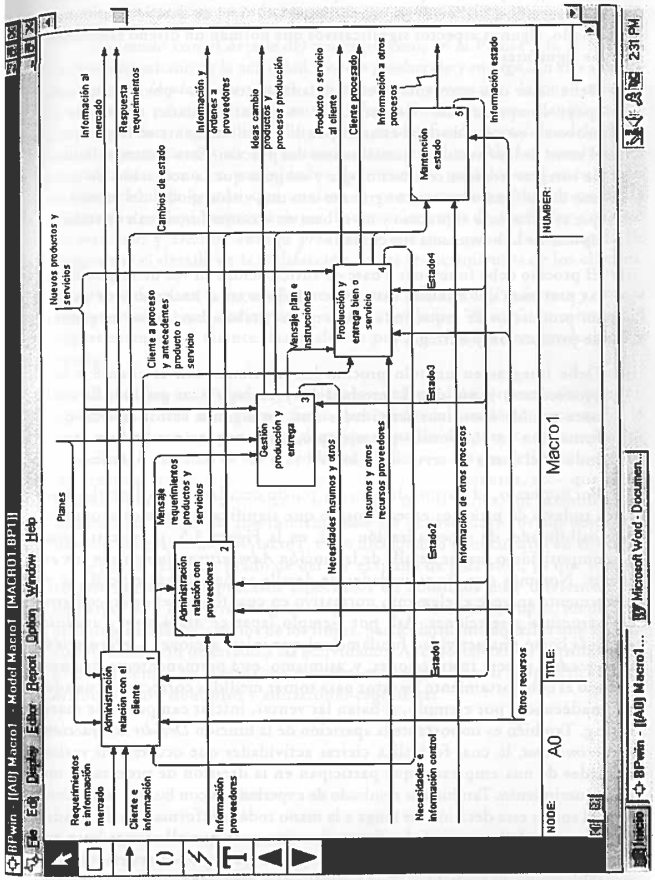
\includegraphics{fig/Macro.png}
\caption{Macro}
\end{figure}

\hypertarget{descripciuxf3n-cuantitativa-de-las-situaciones-en-que-se-trabajaruxe1}{%
\subsubsection{Descripción cuantitativa de las situaciones en que se
trabajará:}\label{descripciuxf3n-cuantitativa-de-las-situaciones-en-que-se-trabajaruxe1}}

identificación, descripción breve, estimación de costos, nivel de
urgencia por cambiar, ¿qué riesgos tiene mantener la situación actual?,
etc.

Duarcon LTDA. es una pequeña empresa\footnote{\url{https://www.economia.gob.cl/wp-content/uploads/2014/04/Boletin-Revision-Clasificacion-Estatuto-Pyme.pdf}
  2021-11-08 20:53:40} dedicada la reparación mecánica y eléctrica
automotriz de vehículos livianos\footnote{Según definición ANAC},
ubicada en Lo Ovalle N 220, Quilicura, cuenta con una plantilla de 6
trabajadores (1 administrador y 5 mecánicos, detallado en la figura
@ref(fig:estruc)). Creada en el ano 2005, ha entregado sus servicios a
la comunidad cercana, su demanda constante del servicio impulso expandir
la plaza de servicio, desde 1000 ft\textsuperscript{2} a 2442
ft\textsuperscript{2}. Debido a la demanda del servicio el año 2009,
Duarcon LTDA. a incorpora a su taller un almacén con un área de 418, con
el propósito de alojar repuestos necesarios en el servicio de
reparación, en el segundo semestre del presente ano Duarcon LTDA., con
el fin agregar a su linea de negocio la venta de neumáticos se construye
otro almacén con un área de 243 ft\textsuperscript{2}, lo que da un
total de 661 ft\textsuperscript{2} de plaza para almacén (vease
@ref(fig:layout)).

\textbf{Label aparte con simbologia}

\begin{figure}
\centering
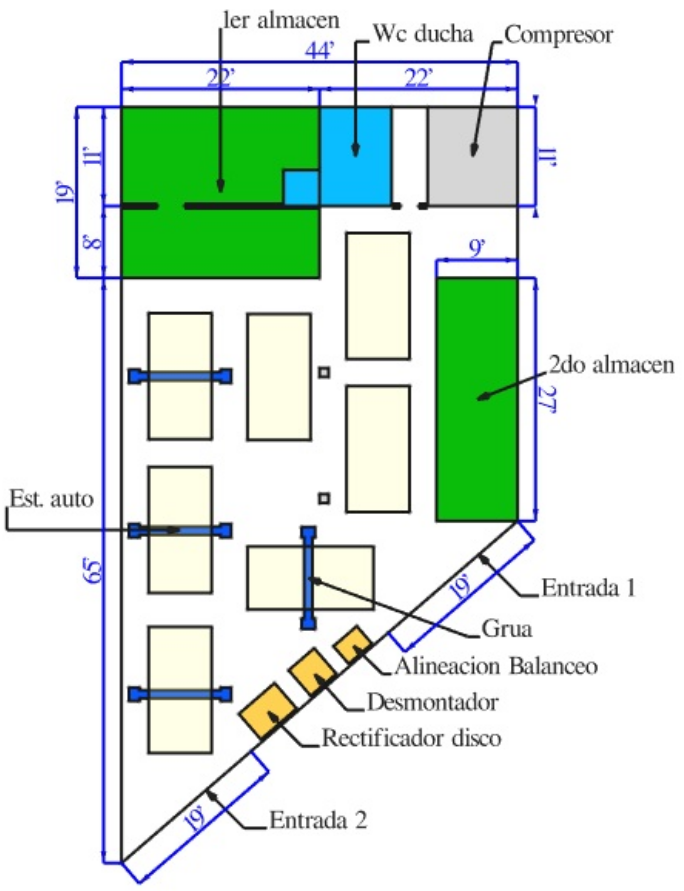
\includegraphics{fig/plan.png}
\caption{plan}
\end{figure}

Para realizar el servicio de reparación automotriz, el mecánico dispone
de repuestos los cuales son solicitados a almacén, el administrador se
encarga en la preparación del repuesto según los siguiente requisitos.

\begin{itemize}
\tightlist
\item
  Tipo repuesto
\item
  Modelo de vehículo
\item
  Cantidad requerida
\end{itemize}

Lo siguiente es ubicar en el los distintos rack el repuesto requerido y
realizar picking\footnote{Sacar el produuuu oe}, para posterior entregar
al mecánico y así continuar con la reparación del vehículo. tal como
detalla la figura @ref(fig:bpmnout).

El proceso mencionado anteriormente \textbf{carese de integridad en la
información}\footnote{calidad informa} por el procedimiento con el que
se realiza la ubicación del repuesto, debido a que no existe registro de
su ubicación, esto tiene relación con el procedimiento al almacenar
recepción, el cual se agrupa según marca de vehículo y se rotular el
packing el producto por modelo, tal como detalla la figura
@ref(fig:bpmnin).

\hypertarget{capitulo-i-definiciuxf3n-del-problema}{%
\section{Capitulo I: Definición del
Problema}\label{capitulo-i-definiciuxf3n-del-problema}}

\hypertarget{problema-y-preguntas-de-investigaciuxf3n}{%
\subsection{Problema y Preguntas de
Investigación}\label{problema-y-preguntas-de-investigaciuxf3n}}

El tema abordado en esta memoria nace de un problema presentado de forma
directa por Duarcon LTDA. que es el desconocimiento del stock, desde
esta base se ha podido hallar otro problema del proceso de gestión de
inventario, como el mencionado anteriormente que es la ubicación del
stock en recepción. Analizaremos el inventario existente, clasificado
según el tipo de repuesto con un costo de \$\textbf{costo invent} pesos,
la variedad de producto es de r lng.ttl.prod y una cantidad total de
stock de r sm.total.in. Para resumir el stock existente la figura
@ref(fig:inventario) se presenta la distribución de frecuencia de
cantidad agrupado según su clasificación

Se puede observar la existencia de sobre stock ejemplo de ello es la
categoría \textbf{categoria} el cual presta un producto con un stock
superior a \textbf{stock max 60} unidades

\hypertarget{justificaciuxf3n-de-la-investigaciuxf3n.---breve-resumen-capitular.}{%
\subsection{Justificación de la Investigación. - Breve Resumen
Capitular.}\label{justificaciuxf3n-de-la-investigaciuxf3n.---breve-resumen-capitular.}}

\textbf{Pendiente cuantificar costoss }

\hypertarget{porque-es-importante-este-proyecto}{%
\subsection{porque es importante este
proyecto}\label{porque-es-importante-este-proyecto}}

Para entender la importancia del inventario, y por que de enfocarse en
ello, se señala que ``el inventario es uno de los activos más costosos
de muchas compañías, llega a representar hasta un 50\% del capital total
invertido.{[}\ldots{]} Por un lado, una empresa puede reducir sus costos
al disminuir el inventario'' {[}@heizer, pp. 484{]}, ademas ``la sola
permanencia de este inventario está generando un sin número de costos
asociados'' {[}@salas2009inventarios, pp. XVI{]}.

\hypertarget{cual-es-la-problemuxe1tica-que-intenta-solucionar}{%
\subsection{cual es la problemática que intenta
solucionar}\label{cual-es-la-problemuxe1tica-que-intenta-solucionar}}

Obtenidos los datos y como se generan, se puede señalar que la
problemática es de tipo metodológico (que implican un método o proceso
estricto para ser solucionados), e involucra al proceso completo desde
la entrada hasta la salida de stock, evidenciando la falta de control
del inventario.

``Las buenas políticas de inventarios pierden sentido si la
administración no sabe qué hay disponible en su inventario'' {[}@heizer,
pp. 486{]}. En consecuencia este sera la problemática a solucionar. Para
la presente proyecto el objetivo es \textbf{mejorar} la gestión de
inventario actual de Duarcon con respecto a la rapidez de y solides de
la información, para ello se propone implementar una herramienta
tecnológica en especifico un software, capas de registrar, controlar y
entregar métodos, técnicas que otorguen al administrador capacidad de
tomar decisiones concretas acerca de pedidos.

\hypertarget{por-que-este-proyecto-y-no-otro}{%
\subsection{por que este proyecto y no
otro}\label{por-que-este-proyecto-y-no-otro}}

La realización de este proyecto es importante debido a que ``Sólo cuando
la organización puede determinar con exactitud qué está disponible es
capaz de tomar decisiones concretas acerca de pedidos, programación y
embarque'', ``La exactitud de los registros permite a las organizaciones
enfocarse en aquellos artículos que son más necesarios, en vez de tener
la seguridad de que ``algo de todo'' está en inventario" {[}@heizer, pp.
486{]}, ademas agregar que el proceso de inventario no agrega valor al
servicio. Se puede inferir que de haber existido un sistema gestión de
inventario, correcto con exactitud en los registros, habría desechado el
\textbf{costo de oportunidad} de realizar de la ampliación de almacén
por utilizar ese espacio en otra estación de reparación.

\hypertarget{formulaciuxf3n-de-hipuxf3tesis.}{%
\subsection{Formulación de
hipótesis.}\label{formulaciuxf3n-de-hipuxf3tesis.}}

\hypertarget{hipuxf3tesis-general}{%
\subsubsection{Hipótesis general}\label{hipuxf3tesis-general}}

La utilización de un sistema tecnológico de manejo y control en la
gestión de inventario herramienta permitirá reducir el espacio necesario
de almacenamiento.

\hypertarget{hipuxf3tesis-especuxedficas}{%
\subsubsection{Hipótesis
específicas}\label{hipuxf3tesis-especuxedficas}}

\begin{itemize}
\tightlist
\item
  Aplicar 5's facilitara la implementación de nuevas mejoras.
\item
  Cuantificar, clasificar el inventario y comparar con la demanda
  visibilizara sobrestock.
\item
  Cuantificar el costo de inventario incentivara el análisis y una
  posterior optimización.
\item
  La implementación de indicadores de gestión permitirá mejora en
  decisiones rápidas en operaciones del almacén.
\item
  La implementación de procedimientos generará una comunicación eficaz
  entre las áreas internas.
\end{itemize}

Para la solución del proceso de gestión de inventario, es necesario
mejorar la metodología en la gestión del almacén, contemplando
distribución, lenguaje iconico \footnote{\url{https://www.diferenciador.com/tipos-de-lenguaje/}},
involucrando métodos y herramientas logísticas, ademas alineado en la
\textbf{industria 4.0} se implementara una herramienta tecnológica que
simplifique la utilización de los métodos y herramientas.

\hypertarget{objetivos-de-la-investigaciuxf3n.}{%
\subsection{Objetivos de la
Investigación.}\label{objetivos-de-la-investigaciuxf3n.}}

\hypertarget{objetivo-general}{%
\subsubsection{Objetivo general:}\label{objetivo-general}}

Mejora de método, herramientas y técnicas que contribuyan en la gestión
y control de inventario del almacén con el fin de proporcionar al
operador de almacén información suficiente para una solida toma de
decisiones y con ello la optimizacion de inventario.

\hypertarget{objetivos-especuxedficos}{%
\subsubsection{Objetivos específicos:}\label{objetivos-especuxedficos}}

\begin{itemize}
\item
  Identificar y analizar, la situación actual de la gestión y control
  del inventario.
\item
  Evaluar la factibilidad de la propuesta de mejora.
\item
  Rediseñar el subproceso de entrada y salida.
\item
  Integrar al rediseño herramienta tecnológica que facilite la ejecución
  del proceso.
\item
  Evaluar los resultados contrastando con la situación actual. \#\#
  Variables de Estudio\footnote{\url{https://psicologiaymente.com/miscelanea/tipos-de-variables}}.
  \#\#\# Variables Dependientes
\item
  Servicio almacén
\end{itemize}

\hypertarget{variables-independientes-intangible}{%
\subsubsection{Variables Independientes
Intangible}\label{variables-independientes-intangible}}

\hypertarget{variables-independientes-tangibles}{%
\subsubsection{Variables Independientes
tangibles}\label{variables-independientes-tangibles}}

\hypertarget{variables-intervinientes}{%
\subsubsection{Variables
Intervinientes}\label{variables-intervinientes}}

\hypertarget{alcance-de-la-investigacion}{%
\subsection{Alcance de la
investigacion}\label{alcance-de-la-investigacion}}

no se tiene acceso a repuestos despachados

\hypertarget{capuxedtulo-ii-marco-teuxf3rico}{%
\section{Capítulo II: MARCO
TEÓRICO}\label{capuxedtulo-ii-marco-teuxf3rico}}

\hypertarget{marco-referente-a-logistica}{%
\subsection{Marco referente a
Logistica}\label{marco-referente-a-logistica}}

La logística es un proceso relacionado con la administración efectiva
del flujo de bienes y servicios. Su operatividad afecta el
desenvolvimiento de muchas áreas de la organización; es por ello que se
puede mencionar de un sistema logístico que mediante la sincronización
de sus componentes, permite lograr el flujo necesario para responder de
manera efectiva a una demanda cambiante y cada vez más exigentes.

Etapas de la logística:

\begin{enumerate}
\def\labelenumi{\arabic{enumi}.}
\tightlist
\item
  Logística de entrada: Planificación, gestión de materiales, alianza
  con los proveedores, negociación, compras y abastecimiento.
\item
  Logística del proceso: Planificación y manejo de recursos.
\item
  Logística de salida: Distribución física y servicio al cliente.
\item
  Supply Chain Management: Gestión de la cadena de valor.
\item
  Logística inversa: Manejo de devoluciones, atención al cliente.
\end{enumerate}

\hypertarget{administraciuxf3n-de-inventario}{%
\subsubsection{Administración de
inventario}\label{administraciuxf3n-de-inventario}}

El objetivo de la administración de inventarios es encontrar un
equilibrio entre la inversión en el inventario y el servicio al cliente.
Sin un inventario bien administrado nunca se podrá lograr una estrategia
de bajo costo {[}@heizer, pp. 484{]} lo cual esta ligado principios del
lean manufacturing.

El inventario puede dar servicio a varias funciones que agregan
flexibilidad a las operaciones de una empresa. Las cuatro funciones del
inventario son:

\begin{enumerate}
\def\labelenumi{\arabic{enumi}.}
\tightlist
\item
  ``Desunir'' o separar varias partes del proceso de producción. Por
  ejemplo, si los suministros de una empresa fluctúan, quizá sea
  necesario un inventario adicional para desunir los procesos de
  producción de los proveedores.
\item
  Separar a la empresa de las fluctuaciones en la demanda y proporcionar
  un inventario de bienes que ofrezca variedad a los clientes. Tales
  inventarios son típicos de los establecimientos minoristas.
\item
  Tomar ventaja de los descuentos por cantidad, porque las compras en
  grandes cantidades pueden reducir el costo de los bienes y su entrega.
\item
  Protegerse contra la inflación y los cambios a la alza en los precios.
\end{enumerate}

\hypertarget{sistema-abc-de-la-clasificaciuxf3n-de-inventarios}{%
\paragraph{Sistema ABC de la clasificación de
inventarios}\label{sistema-abc-de-la-clasificaciuxf3n-de-inventarios}}

El análisis ABC divide el inventario disponible en tres clases con base
en su volumen anual en dinero, la figura @ref(fig:ABC) representa este
análisis. El análisis ABC es una aplicación a los inventarios de lo que
se conoce como principio de Pareto. El principio de Pareto establece que
hay ``pocos artículos cruciales y muchos triviales''\footnote{Vilfredo
  Pareto, economista italiano del siglo XIX}. La idea es establecer
políticas de inventarios que centren sus recursos en las pocas partes
cruciales del inventario y no en las muchas partes triviales. No es
realista monitorear los artículos baratos con la misma intensidad que a
los artículos costosos {[}@heizer, pp. 485{]}. Ademas se afirma que ``si
se aplican en forma selectiva políticas de inventarios a estos
diferentes grupos, pueden lograrse, con niveles más bajos de
inventarios, los objetivos del servicio de inventarios, en vez de una
política aplicada colectivamente a todos los productos'' {[}@logist, pp.
376{]}.

\begin{figure}
\centering
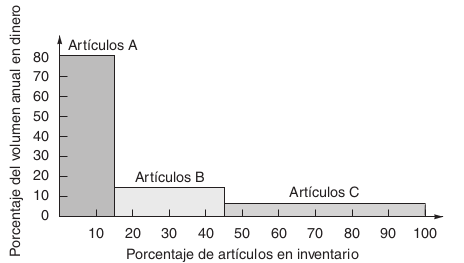
\includegraphics{fig/abcteo.png}
\caption{abcteo}
\end{figure}

\hypertarget{conteo-cuxedclico-o-inventario}{%
\paragraph{Conteo cíclico o
``inventario''}\label{conteo-cuxedclico-o-inventario}}

Aunque una organización haya realizado esfuerzos sustanciales para
registrar con precisión su inventario, los registros deben verificarse
mediante una auditoría continua. El conteo cíclico usa la clasificación
del inventario desarrollada en el análisis ABC. Con los procedimientos
de conteo cíclico, se cuentan los artículos, se verifican los registros,
y se documentan las imprecisiones de manera periódica. Se rastrea la
causa de las imprecisiones y se toman las acciones correctivas
apropiadas para asegurar la integridad del sistema de inventario. La
frecuencia de conteo depende del tipo de producto de mayor a menor los
artículos, A,B,C respectivamente {[}@heizer, pp. 487{]}

\hypertarget{warehouse}{%
\subsubsection{Warehouse}\label{warehouse}}

Un almacén controla el ingreso y salida de materiales, por lo tanto es
importante tener codificados todos los productos, definir correctamente
las unidades y clasificar los ítems. Según Cachay (2010) es definido
``Proceso de la función logística que trata la recepción, almacenamiento
y movimiento dentro de un mismo almacén hasta el punto de consumo de
cualquier material, así como el tratamiento e información de los datos
generados''.

El proceso de planificación, organización y gestión de almacenes está a
cargo de la gerencia o jefatura, alcanza las actividades de carácter
estratégico y táctico. Estas actividades contempla:

\begin{enumerate}
\def\labelenumi{\arabic{enumi}.}
\item
  Diseño de la red de distribución y almacenamiento
\item
  Responsabilidades de la gestión de almacenes:
\item
  Ubicación de los almacenes: Las decisiones sobre ubicación implican de
  determinar el número, ubicación y tamaño de las instalaciones que se
  utilizarán.
\item
  Diseño y Layout de los almacenes: Corresponde a la disposición de los
  elementos dentro del almacén.
\item
  Modelo de organización física de los almacenes:

  \begin{itemize}
  \tightlist
  \item
    Determinar las ubicaciones de existencias y establecer el sistema de
    almacenamiento.
  \item
    Establecer el sistema de manejo de materiales.
  \item
    Mantener un sistema de control de inventarios.
  \item
    Establecer procedimientos para tramitar los pedidos.
  \item
    Seleccionar el medio de transporte.
  \end{itemize}
\end{enumerate}

Como primicia, la propuesta de esta investigación es la implementación
de un métodos de control en la gestión de inventario mediante un
software WMS, por lo que respecta a la construcción del software se
analizara de forma general sin caer en demasiado tecnicismos, se
incluirá información acerca de su funcionamiento, debido a que es un
proyecto para el titulo de la carrera ingeniero civil industrial.

Con respecto a lo anterior se ha consultado proyectos con un objetivo
similar de la implementación de un software, pero propuesto por un
ingeniero ajeno a la ingeniería informática, con el objetivo de
visibilizar la nula limitante de este tipo de propuesta, ademas
esperando ser un aporte se agrega que el desarrollo de software es
realizado por el autor de este proyecto con los conocimientos adquiridos
en la carrera ademas de fruto de investigación estos conocimientos
comprenden, estadística, logística, proceso, informática.

La problemática de la organización, la cual radica en el método
utilizado para la gestión de inventario se presenta algunos conceptos y
teorías que se enfocan en \textbf{Rediseño de procesos},
\textbf{Administración de inventario}, y desarrollo software en
especifico \textbf{desarrollo web}, para lo cual se mencionaran
estrategias y metodología que posibiliten la solución al del problema
del almacén, también se menciona la industria 4.0 debido a que se
plantea como un modelo actual que reconoce la evolución de la industria
en torno a la tecnología.

Para crear el puente a la construcción de software se utilizara la
teoría de Oscar Barros el autor propone en su libro que los procesos
típicos de todas las organizaciones son pocos y las prácticas para
ejecutar dichos procesos no difieren mucho. Es por esto que se puede
modelar una estructura general para cada uno de ellos y luego ser
aplicada a un dominio específico.

\hypertarget{marco-referente-a-rediseuxf1o-de-procesos}{%
\subsection{Marco referente a rediseño de
procesos}\label{marco-referente-a-rediseuxf1o-de-procesos}}

El rediseño de procesos consiste en tomar las actividades de un proceso
en su totalidad y someterlas a un cambio fundamental, el cual
habitualmente implica un uso intensivo de Tecnologías de la Información
que garantice un desempeño claramente mejorado del mismo {[}@proce, pp.
14{]}, ademas concluye que ``en cualquier organización hay un numero
pequeño de tipos de procesos y cada uno de ellos ademas, de tener una
arquitectura o estructura común que comparte con los otros es muy
parecido en su esencia en diferentes contextos, a esta estructura común
le denomina \textbf{Patrón de proceso}'' {[}@proce, pp. 17{]}. para esto
define el concepto de \textbf{Macroproceso} ``como un conjunto de
procesos que podemos ligar naturalmente y que en algunas situaciones
ocurren en forma totalmente interrelacionada'' {[}@proce, pp. 21{]}.
Coincide con este análisis el Trabajo estándar {[}@leanmanu, pp. 297{]}
que tiene su fundamento en la excelencia operacional, sin el trabajo
estandarizado no se puede garantizar que en las operaciones siempre se
elaboren los productos de la misma manera. El trabajo estandarizado hace
posible aplicar los elementos de Lean Manufacturing (se interiorizara
mas adelante) ya que define de la manera mas eficiente los métodos de
trabajo para lograr la mejor calidad y los costos mas bajos".

Es así como se definen 4 macroprocesos que se muestran a continuación:

\hypertarget{definiciuxf3n-macroprocesos}{%
\subsubsection{Definición
Macroprocesos}\label{definiciuxf3n-macroprocesos}}

\begin{enumerate}
\def\labelenumi{\arabic{enumi}.}
\item
  Macroproceso 1, de gestión, producción y provisión del bien o
  servicio: Se define como aquel que ``representa la cadena integral del
  valor de una empresa, parte desde que se genera el requerimiento del
  cliente, pasando por la obtención de factores ofrecidos por los
  proveedores, producción del bien o servicio y entrega al cliente
  final. Referida a las cadenas de abastecimientos (supply chain) de una
  organización'' {[}@proce, pp. 22{]}
\item
  Macroproceso 2, desarrollo de nuevos productos y/o servicios:
  ``contiene el conjunto de actividades, que muchas veces se encuentran
  dispersas en diferentes áreas funcionales, que permiten descubrir,
  definir, evaluar, diseñar, probar e implementar nuevos bienes o
  servicios en una compañía'' {[}@proce, pp. 23{]}. Su propósito es
  innovar incrementando la oferta a los clientes y generar ventajas
  competitivas.
\item
  Macroproceso 3 Planificación de negocio: ``Son todas aquellas
  actividades a nivel táctico y estratégico que buscan establecer
  políticas, planes, programas u orientaciones buscando guiar el destino
  de la empresa a futuro (mediano o largo plazo)'' {[}@proce, pp. 25{]}.
  Estas actividades son: Definición del negocio, Estructura del negocio,
  Planificación mediano-largo plazo.
\item
  Macroproceso 4 de apoyo: Ciclo de vida de un recurso Contiene el
  conjunto de actividades que tienen como propósito ejecutar el ciclo de
  vida de los recursos y su funcionamiento. Consiste en detectar
  necesidades, obtener, asignar y designar recursos humanos,
  financieros, de materiales, insumos, infraestructura, entre otros
  {[}@proce, pp. 29{]}.
\end{enumerate}

\hypertarget{modelamiento-de-procesos}{%
\subsubsection{Modelamiento de
procesos}\label{modelamiento-de-procesos}}

La interacción entre los macroprocesos se da a través de flujos que
representan como un macroproceso se alimenta y requiere servicios de los
otros macroprocesos. Para el modelamiento de procesos se propone la
utilizacion de los diagramas de flujos y patrones conocida como IDEFO
(Integration Definition for Function Modeling) {[}@proce, pp. 34{]} la
figura @ref.

\begin{figure}
\centering
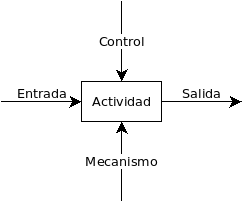
\includegraphics{fig/modelamientoestructurado.png}
\caption{modelamientoestructurado}
\end{figure}

\hypertarget{metodologuxeda-de-rediseuxf1o-mediante-el-uso-de-patrones}{%
\subsubsection{Metodología de rediseño mediante el uso de
patrones}\label{metodologuxeda-de-rediseuxf1o-mediante-el-uso-de-patrones}}

Barros propone dos metodologías para realizar reingeniería o rediseño de
procesos, resumidas indican que:

\begin{enumerate}
\def\labelenumi{\arabic{enumi}.}
\item
  Propuesta originalmente por \textbf{Hammer}, enfatiza en la ``idea
  empezar de cero'' lo cual implica repensar sin prejuicio histórico, el
  proceso en cuestión.
\item
  Propone partir de un conocimiento profundo del proceso actualmente
  existente, a partir de esto generar una propuesta de rediseño.
\end{enumerate}

de lo anterior adapta la metodología propuestas en el libro Reingeniería
de Procesas de Negocios {[}@proce, pp. 97{]}, que se presenta resumido
en la figura @ref(fig:metoredi)

\begin{figure}[H]

{\centering 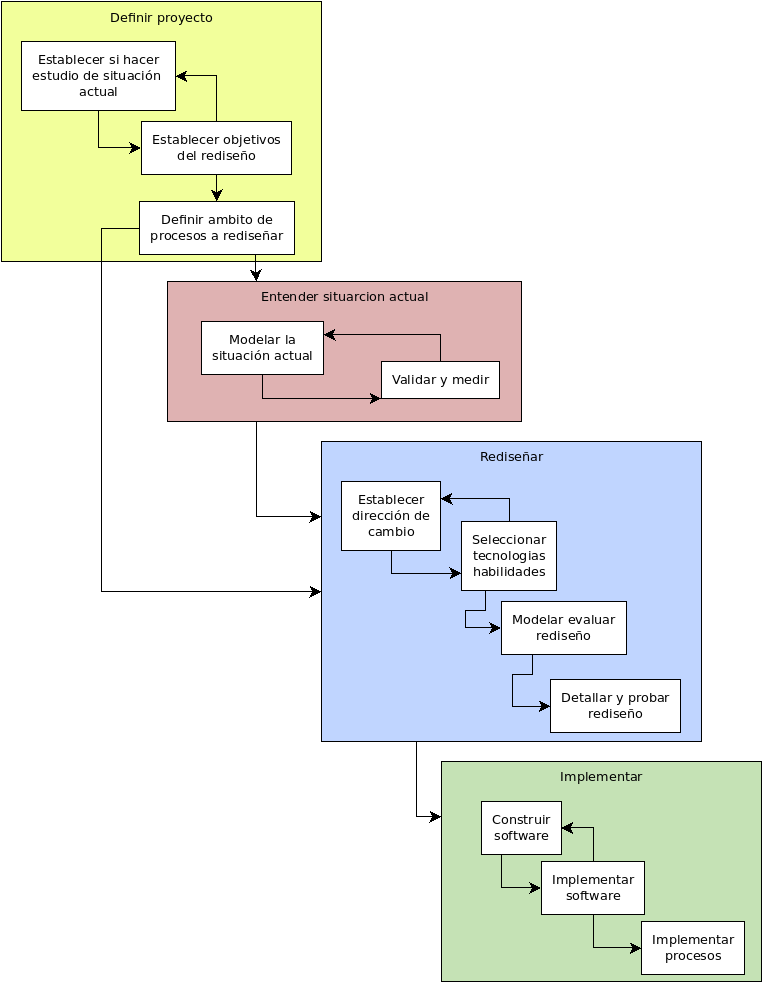
\includegraphics[width=0.8\linewidth]{marco teorico/diagramas/metologia_rediseno} 

}

\caption{Metodología rediseño}\label{fig:unnamed-chunk-1}
\end{figure}

\hypertarget{marco-referente-a-muxe9todos-filosofias-herramientas.}{%
\subsection{Marco referente a métodos, filosofias,
herramientas.}\label{marco-referente-a-muxe9todos-filosofias-herramientas.}}

Esta sección del marco se basa en la teoría del libro ``Lean
Manufacturing paso a paso'' del autor Luis Socconini el cual presenta
las diferentes herramientas y técnicas que contribuirán con el objetivo
de la propuesta, estas se clasifican de la siguiente manera:

\begin{enumerate}
\def\labelenumi{\arabic{enumi}.}
\tightlist
\item
  Herramientas básicas

  \begin{itemize}
  \tightlist
  \item
    5's
  \item
    Andon, Control visual
  \end{itemize}
\item
  Herramientas para mejorar la calidad

  \begin{itemize}
  \tightlist
  \item
    AMEF, análisis de modo y efecto de falla
  \item
    Poka Yoke, a prueba de errores
  \end{itemize}
\end{enumerate}

\hypertarget{industria-4.0}{%
\subsubsection{Industria 4.0}\label{industria-4.0}}

El término industria 4.0 se refiere a un nuevo modelo de organización y
de control de la cadena de valor a través del ciclo de vida del producto
y a lo largo de los sistemas de fabricación apoyado y hecho posible por
las tecnologías de la información. El término industria 4.0 se utiliza
de manera generalizada en Europa, si bien se acuñó en Alemania. También
es habitual referirse a este concepto con términos como ``Fábrica
Inteligente'' o ``Internet industrial''. En definitiva se trata de la
aplicación a la industria del modelo ``Internet de las cosas'' (IoT).
Todos estos términos tienen en común el reconocimiento de que los
procesos de fabricación se encuentran en un proceso de
\textbf{transformación digital}, una ``revolución industrial'' producida
por el avance de las tecnologías de la información, particularmente de
la informática y el software {[}@indust4{]}.

\hypertarget{filosofuxeda-lean-manufacturing}{%
\subsubsection{Filosofía Lean
Manufacturing}\label{filosofuxeda-lean-manufacturing}}

``Se puede define como un proceso continuo y sistemático de
identificación y eliminación del desperdicio o excesos, entendiendo como
exceso toda aquella actividad que no agrega valor en un proceso, pero si
costo y trabajo. Esta eliminación sistemática se lleva a cabo mediante
trabajo con equipos de personas bien organizados y
capacitados''{[}@leanmanu, pp. 11{]}.

{[}@leanmanu, pp. 15{]} Agrega que el éxito no basta con introducir
nuevas metodologías y herramientas para que las empresas logren cambios
significativos, el reto consiste realmente en modificar de manera
positiva la cultura. Se establecen tres tópicos para el éxito:
participación, herramientas, cultura. figura @ref(fig:exito).

Falta de estos tópicos del éxito tiene como consecuencia en la
productividad {[}@leanmanu, pp. 26{]}. Lean manufacturing visibiliza las
limitantes de la productividad, los ingenieros japoneses han clasificado
estas limitantes en tres grupos a los que llamaron las 3 ``Mu'', debido
a que todas inician con la silaba mu:

\begin{figure}

{\centering 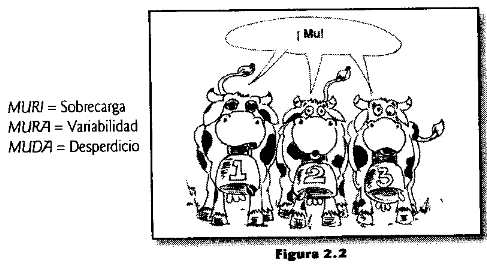
\includegraphics[width=0.5\linewidth]{marco teorico/Screenshot from 2021-11-02 00-44-42} 

}

\caption{Tres limitantes de la productividad}\label{fig:unnamed-chunk-2}
\end{figure}

\hypertarget{principios-en-los-que-se-basa-la-filosofuxeda-lean-manufacturing}{%
\paragraph{Principios en los que se basa la filosofía Lean
Manufacturing:}\label{principios-en-los-que-se-basa-la-filosofuxeda-lean-manufacturing}}

\begin{itemize}
\tightlist
\item
  Hacer sólo ``lo que es necesario, cuando es necesario, y en la
  cantidad necesaria''.
\item
  La calidad debe ser parte inherente del proceso.
\item
  El tiempo total de proceso (Lead Time) debe ser mínimo.
\item
  Se debe alcanzar una alta utilización de máquinas y mano de obra.
\item
  Mejora Continua.
\end{itemize}

\hypertarget{herramientas-basicas}{%
\subsubsection{Herramientas basicas}\label{herramientas-basicas}}

\hypertarget{s}{%
\paragraph{5's}\label{s}}

Las 5's constituyen una disciplina para lograr mejoras en la
productividad del lugar de trabajo mediante la estandarización de
hábitos de orden y limpieza. Representa una de las piedras que enmarcan
el inicio de cualquier herramienta o sistema de mejora. Por ello, se
dice que un buen evento de mejora es aquel que se inicia con las 5's.
Esto se logra implementando cambios en los procesos en cinco etapas,
cada una de las cuales servirá de Fundamento a la siguiente, para así
mantener sus beneficios en el largo plazo {[}@leanmanu, pp. 147{]}
@ref(tab:5s)

Se dice que si en una empresa no ha funcionado la implementación de las
5's, cualquier otro sistema de mejoramiento de los procesos esté
destinado a fracasar. Esto se debe a que no se requiere tecnología ni
conocimientos especiales para implementarlas, solo \textbf{disciplina y
autocontrol} por parte de cada uno de los miembros de la organización.

\hypertarget{andon-control-visual}{%
\paragraph{Andon, control visual}\label{andon-control-visual}}

El trabajo se relaciona con simples señales visuales y de audio que se
identifican y entienden con facilidad, estas señales son eficientes,
autorreguladas y las manejan los operadores. Esta información se puede
utilizar para identificar, instruir indicar que existe una condición
normal o anormal y que se puede requerir alguna acción.

Andon es un elemento del principio Jidoka\footnote{El Método Jidoka es
  una metodología japonesa incluida en Lean Manufacturing, la cual busca
  que cada proceso tenga su propio autocontrol de calidad (refiriéndose
  principalmente a procesos industriales de producción en linea o a gran
  escala).} que, mediante ingeniosos mecanismos, detecta cuando ocurre
una Falla y entonces, con una señal generalmente visual, avisa al
operador que se ha generado un problema, Andon es una señal que
incorpora elementos visuales, auditivos y de texto que sirven para
notificar problemas de calidad o paros por ciertos motivos. Proporciona
información en tiempo real y retroalimentación del estado de un proceso,

\begin{figure}

{\centering 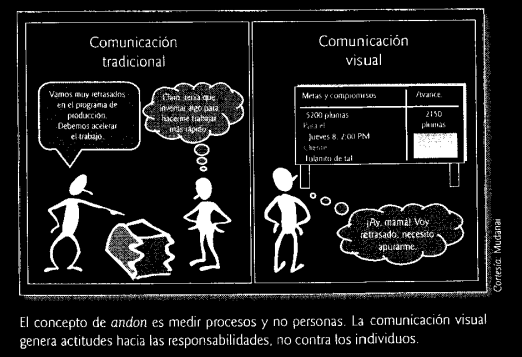
\includegraphics[width=0.5\linewidth]{marco teorico/Screenshot from 2021-11-02 17-19-42} 

}

\caption{concepto de andon es medir pfocesos y no personas, La Comunicaclén visual genera acutudes hacia las responsabilidades, no contra los individuos}\label{fig:unnamed-chunk-3}
\end{figure}

\hypertarget{herramienta-de-calidad}{%
\subsubsection{Herramienta de calidad}\label{herramienta-de-calidad}}

\hypertarget{amef-analisis-de-modo-y-efecto-de-fallas}{%
\paragraph{AMEF, Analisis de modo y efecto de
fallas}\label{amef-analisis-de-modo-y-efecto-de-fallas}}

"Herramienta muy poderosa que permite identificar fallas en productos y
procesos y evaluar objetivamente sus efectos, causas y elementos de
detección para evitar su ocurrencia y tener un método documentado de
prevencion. El AMEF es un documento vivo en el que podemos almacenar una
gran cantidad de datos sobre nuestros procesos y productos, por lo que
constituye una Fuente invaluable de información {[}@leanmanu, pp.
223{]}.

Se identifican los siguientes tipos de AMEF:

\begin{itemize}
\tightlist
\item
  Producto: Sirve para detectar posibles fallas en el diseño de
  productos y anticiparse al efecto que puedan tener en el usuario o
  proceso de fabricación.
\item
  Proceso: Es un análisis de las Fallas que pueden suceder en cada etapa
  del proceso y se utiliza para prevenir que esas fallas tengan efectos
  negativos en el usuario del producto o servicio o en etapas
  posteriores del proceso.
\item
  Sistemas: Se utiliza en el d\textbar seno del software para anticipar
  fallas en su funcionamiento.
\item
  Varios: Existen AMEF para muchos otros tipos de fallas que generen
  efectos negativos y cuyas causas deban documentarse para anticipar
  problemas.
\end{itemize}

\hypertarget{poka-yoke-a-prueba-de-errores}{%
\paragraph{Poka yoke, a prueba de
errores}\label{poka-yoke-a-prueba-de-errores}}

Los dispositivos Poka Yoke son métodos que evitan los errores humanos en
los procesos antes de que se conviertan en defectos, y permiten que los
operadores se concentren en sus actividades. Los Sistemas Poka Yoke
permiten realizar la inspección al 100\% y, por ende, tomar acciones
inmediatas cuando se presentan defectos.

Las siguientes son algunas de las utilidades de implementar Poka Yoke:

\begin{itemize}
\tightlist
\item
  Asegura la calidad en cada puesto de trabajo.
\item
  Proporciona a los operadores conocimiento sobre las operaciones.
\item
  Elimina o reduce la posibilidad de cometer errores.
\item
  Evita accidentes causados por distracción humana.
\item
  Elimina acciones que dependen de la memoria y la inspección.
\item
  Libera la mente del trabajador y le permite desarrollar su creatividad
\item
  Generalmente los Sistemas Poka Yoke son baratos y sencillos.
\end{itemize}

\hypertarget{marco-al-proceso-de-desarrollo-del-software}{%
\subsection{Marco al proceso de desarrollo del
software}\label{marco-al-proceso-de-desarrollo-del-software}}

Un proceso de desarrollo de software tiene como propósito la producción
eficaz y eficiente de un producto software que reúna los requisitos del
cliente. Dicho proceso, en términos globales se muestra en la Figura
@ref(fig:soft\_proc) \footnote{Jacaboson, I., Booch, G., Rumbaugh J., El
  Proceso Unificado de Desarrollo de Software, Addison Wesley 2000.}.
Este proceso es intensamente intelectual, afectado por la creatividad y
juicio de las personas involucradas\footnote{Sommerville, I., Ingeniería
  de Software, Pearson Educación, 2002.}. Aunque un proyecto de
desarrollo de software es equiparable en muchos aspectos a cualquier
otro proyecto de ingeniería, en el desarrollo de software hay una serie
de desafíos adicionales, relativos esencialmente a la naturaleza del
producto obtenido. \footnote{\url{https://revistas.utp.ac.pa/index.php/ric/article/view/1252/html}}

\begin{figure}

{\centering 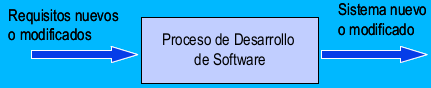
\includegraphics[width=0.5\linewidth]{marco teorico/Screenshot from 2021-11-09 04-03-10} 

}

\caption{Proceso de desarrollo de software}\label{fig:unnamed-chunk-4}
\end{figure}

El proceso de desarrollo de software no es único. No existe un proceso
de software universal que sea efectivo para todos los contextos de
proyectos de desarrollo. Debido a esta diversidad, es difícil
automatizar todo un proceso de desarrollo de software. A pesar de la
variedad de propuestas de proceso de software, existe un conjunto de
actividades fundamentales que se encuentran presentes en todos ellos
\footnote{Sommerville, I., Ingeniería de Software, Pearson Educación,
  2002.}: 1. Especificación de software: Se debe definir la
funcionalidad y restricciones operacionales que debe cumplir el
software. 2. Diseño e Implementación: Se diseña y construye el software
de acuerdo a la especificación. 3. Validación: El software debe
validarse, para asegurar que cumpla con lo que quiere el cliente. 4.
Evolución: El software debe evolucionar, para adaptarse a las
necesidades del cliente.

\hypertarget{tipo-de-programa}{%
\subsubsection{Tipo de programa}\label{tipo-de-programa}}

A través de los años, la logística ha sufrido importantes
transformaciones no sólo en términos conceptuales sino también cómo ha
evolucionado a lo que conocemos hoy día como e-logística, con lo cual se
incorpora la utilización de una herramienta fundamental como es
Internet. Debido a este avance, las organizaciones han determinado un
cambio en su manejo de inventarios, almacenes y cadena de suministro.
Dando esto como resultado las implementaciones de ciertos sistemas de
apoyo como WMS, SCM, ERP y CRM.

\hypertarget{modelo-de-desarrollo}{%
\subsubsection{Modelo de desarrollo}\label{modelo-de-desarrollo}}

Desarrollo evolutivo La idea detrás de este modelo es el desarrollo de
una implantación del sistema inicial, exponerla a los comentarios del
usuario, refinar en N versiones hasta que se desarrolle el sistema
adecuado. En la Figura 6 se observa cómo las actividades concurrentes:
especificación, desarrollo y validación, se realizan durante el
desarrollo de las versiones hasta llegar al producto final. Una ventaja
de este modelo es que se obtiene una rápida realimentación del usuario,
ya que las actividades de especificación, desarrollo y pruebas se
ejecutan en cada iteración. @ref(fig:sftproc)

\begin{figure}

{\centering 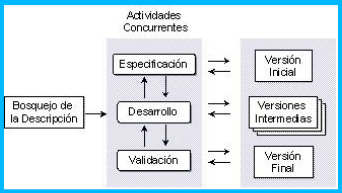
\includegraphics[width=0.5\linewidth]{marco teorico/Screenshot from 2021-11-09 04-24-09} 

}

\caption{Modelo desarrollo evolutivo de software}\label{fig:unnamed-chunk-6}
\end{figure}

Existen dos tipos de desarrollo evolutivo:

\begin{itemize}
\tightlist
\item
  Desarrollo Exploratorio: El objetivo de este enfoque es explorar con
  el usuario los requisitos hasta llegar a un sistema final. El
  desarrollo comienza con las partes que se tiene más claras. El sistema
  evoluciona conforme se añaden nuevas características propuestas por el
  usuario.
\item
  Enfoque utilizando prototipos: El objetivo es entender los requisitos
  del usuario y trabajar para mejorar la calidad de los requisitos. A
  diferencia del desarrollo exploratorio, se comienza por definir los
  requisitos que no están claros para el usuario y se utiliza un
  prototipo para experimentar con ellos. El prototipo ayuda a terminar
  de definir estos requisitos.
\end{itemize}

Este modelo es efectivo en proyectos pequeños (menos de 100.000 líneas
de código) o medianos (hasta 500.000 líneas de código) con poco tiempo
para su desarrollo y sin generar documentación para cada versión.

\hypertarget{metodologuxedas-para-desarrollo-de-software}{%
\subsubsection{Metodologías para desarrollo de
software}\label{metodologuxedas-para-desarrollo-de-software}}

Metodologías ágiles Un proceso es ágil cuando el desarrollo de software
es incremental (entregas pequeñas de software, con ciclos rápidos),
cooperativo (cliente y desarrolladores trabajan juntos constantemente
con una cercana comunicación), sencillo (el método en sí mismo es fácil
de aprender y modificar, bien documentado), y adaptable (permite
realizar cambios de último momento).

\hypertarget{back}{%
\subsubsection{Back}\label{back}}

\hypertarget{phpmyadmin}{%
\paragraph{phpMyAdmin}\label{phpmyadmin}}

\hypertarget{base-de-datos-modelo-relacional}{%
\paragraph{Base de datos, modelo
relacional}\label{base-de-datos-modelo-relacional}}

MySQL es un sistema de gestión de base de datos relacional, multihilo y
multiusuario; incluye todos los elementos necesarios para instalar el
programa, preparar diferentes niveles de acceso de usuario, administrar
el sistema y proteger los datos, puede desarrollar sus propias
aplicaciones de bases de datos en la mayor parte de lenguajes de
programación utilizados en la actualidad y ejecutarlos en casi todos los
sistemas operativos. MySQL es una base de datos robusta que puede ser
comparada con una base de datos comercial, compite con sistemas RDBMS
propietarios como Oracle, SQL Server y DB2, disponiendo de procesamiento
de transacciones a través del motor de almacenamiento InnoDb compatible
con ACID y, que dispone de procedimientos almacenados, triggers, y
vistas.\\
MySQL es lo suficientemente flexible para trabajar en entornos con gran
demanda, tales como aplicaciones web; al mismo tiempo, puede impulsar
aplicaciones empotradas, almacenes de datos, indexación de contenidos,
sistemas de mensajería, sistemas redundantes de alta disponibilidad,
procesamiento de transacciones en línea (OLTP), y mucho más.

\hypertarget{r12}{%
\paragraph[R]{\texorpdfstring{R\footnote{\url{https://cran.r-project.org/doc/contrib/rdebuts_es.pdf}}}{R}}\label{r12}}

R es un sistema para análisis estadísticos y gráficos creado por Ross
Ihaka y Robert Gentleman. R se distribuye gratuitamente bajo los
términos de la GNU General Public Licence, su desarrollo y distribución
son llevados a cabo por varios estadísticos conocidos como el Grupo
Nuclear de Desarrollo de R.

\hypertarget{php}{%
\paragraph{php}\label{php}}

PHP, cuyas siglas responden a un acrónimo recursivo (PHP: hypertext
preprocessor), es un lenguaje sencillo, de sintaxis cómoda y similar a
la de otros lenguajes como Perl, C y C++. Es rápido, interpretado,
orientado a objetos y multiplataforma. Para él se encuentra disponi- ble
una multitud de librerías. PHP es un lenguaje ideal tanto para
Desarrollo de aplicaciones web aprender a desarrollar aplicaciones web
como para desarrollar apli- caciones web complejas. PHP añade a todo eso
la ventaja de que el intérprete de PHP, los diversos módulos y gran
cantidad de librerías desarrolladas para PHP son de código libre, con lo
que el programa- dor de PHP dispone de un impresionante arsenal de
herramientas li- bres para desarrollar aplicaciones. PHP suele ser
utilizado conjuntamente con Perl, Apache, MySQL o PostgreSQL en sistemas
Linux, formando una combinación barata (todos los componentes son de
código libre), potente y versátil. Tal ha sido la expansión de esta
combinación que incluso ha merecido conocerse con un nombre propio LAMP
(formado por las iniciales de los diversos productos)

\hypertarget{end}{%
\subsubsection{End}\label{end}}

\hypertarget{js}{%
\paragraph{js}\label{js}}

Javascript es un lenguaje de programación interpretado (un lenguaje de
tipo script). A pesar de que existen intérpretes no dependientes de
ningún navegador, es un lenguaje de script que suele encontrarse
vinculado a páginas web, es utilizado para hacer

\hypertarget{html}{%
\subsubsection{html}\label{html}}

El lenguaje HTML ( hypertext markup language ) se utiliza para crear
documentos que muestren una estructura de hipertexto. Un documento de
hipertexto es aquel que contiene información cruzada con otros
documentos, lo cual nos permite pasar de un documento al referenciado
desde la misma aplicación con la que lo estamos visualizando.

\hypertarget{css}{%
\subsubsection{css}\label{css}}

\newpage

\hypertarget{capuxedtulo-iii-diseuxf1o-metodoluxf3gico}{%
\section{Capítulo III: DISEÑO
METODOLÓGICO}\label{capuxedtulo-iii-diseuxf1o-metodoluxf3gico}}

\hypertarget{enfoque}{%
\subsection{Enfoque}\label{enfoque}}

El debido a la naturaleza de la propuesta de rediseño de proceso se
puede establecer que la presente investigación tiene un enfoque
cuantitativo, por su necesidad de un análisis numérico del stock, el
alcance del trabajo sera de campo debido a que se realizara en el
almacén. De carácter descriptivo debido a la observación que se incurre
en el rediseno de proceso, también se describe como una investigación
aplicativa por el objetivo de resolver un problema utilizando el
conocimiento e implementar de forma practica, para satisfacer
necesidades concretas\footnote{\url{http://www2.duoc.cl/biblioteca/crai/definicion-y-proposito-de-la-investigacion-aplicada}
  La Investigación Aplicada tiene por objetivo resolver un determinado
  problema o planteamiento específico, enfocándose en la búsqueda y
  consolidación del conocimiento para su aplicación y, por ende, para el
  enriquecimiento del desarrollo cultural y científico.}.

\hypertarget{diseuxf1o.}{%
\subsection{Diseño.}\label{diseuxf1o.}}

Para realizar la propuesta de mejora en el proceso de gestión de almacén
se utilizara la teoría de Oscar Barros añadiendo la filosofía de lean
manufacturing. Como principio se utilizara para este caso especifico la
variante metodológica de rediseño, que contempla como referencia la
situación actual, por tanto la propuesta del diseno de la metodología en
general contara con las etapas que describe la figura
@ref(fig:metoredi).

\begin{figure}

{\centering 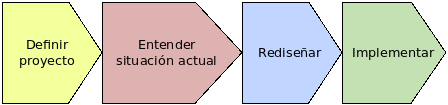
\includegraphics[width=0.5\linewidth]{marco teorico/diagramas/metodo_resu} 

}

\caption{Metodología general}\label{fig:unnamed-chunk-7}
\end{figure}

\hypertarget{contexto}{%
\subsection{Contexto}\label{contexto}}

El presente proyecto su realización en Duarcon LTDA. ubicado en Lo
Ovalle N 220, Quilicura, el periodo de investigación contempla Enero del
2021 a Mayo de 2021

\hypertarget{operacionalizaciuxf3n-de-las-variables.}{%
\subsection{Operacionalización de las
variables.}\label{operacionalizaciuxf3n-de-las-variables.}}

A continuación se establecen y describen las variables que comprende la
propuesta:

\hypertarget{variable-dependiente}{%
\subsubsection{Variable dependiente:}\label{variable-dependiente}}

\hypertarget{capacidad-necesaria-de-almacuxe9n}{%
\paragraph{Capacidad necesaria de
almacén}\label{capacidad-necesaria-de-almacuxe9n}}

La construcción de un nuevo almacén en el taller por falta de espacio
debido a un posible sobre stock de repuesto, requiere de un análisis de
espacio necesario para el almacenaje de repuesto. En consecuencia la
optimizacion de esta variable osea reducir capacidad de almacenamiento
necesario de stock es primordial, por lo tanto se propone como variable
dependiente la cual se ve afecta por las siguientes variables
independientes

\hypertarget{variables-independientes-intangible-1}{%
\subsubsection{Variables Independientes
Intangible}\label{variables-independientes-intangible-1}}

\hypertarget{variables-independientes-tangibles-1}{%
\subsubsection{Variables Independientes
tangibles}\label{variables-independientes-tangibles-1}}

\hypertarget{volumen-packing-por-repuesto}{%
\paragraph{Volumen packing por
repuesto}\label{volumen-packing-por-repuesto}}

Se considera la medidas de la caja del repuesto. \#\#\#\# Cantidad total
por repuesto Esta variable contempla la cantidad total por repuesto
\#\#\#\# Merma Esta variable se cuantifica de la existencia teórica con
respecto a la existencia real \#\#\#\# Tecnología o método de control.
Herramienta o método de control utilizado para la gestión de inventario

\hypertarget{poblaciuxf3n-y-muestra.}{%
\subsection{Población y Muestra.}\label{poblaciuxf3n-y-muestra.}}

La población es el inventario total y la muestra una ubicación en
particular

\hypertarget{recolecciuxf3n-de-datos.}{%
\subsection{Recolección de datos.}\label{recolecciuxf3n-de-datos.}}

\begin{itemize}
\tightlist
\item
  entrevista encargado
\item
  revisión de registro de facturas recepción
\item
  Medir, la instalaciones
\item
  observación, del proceso actual, desorden
\item
  prueba, preguntar ubicación de productos
\item
  conteo de inventario,
\end{itemize}

\hypertarget{plan-de-anuxe1lisis.}{%
\subsection{Plan de análisis.}\label{plan-de-anuxe1lisis.}}

Para términos de alcance de la presente memoria, se propone enfocar el
trabajo en las etapas 1, 2 y 3, dejando de lado la implementación, pero
sí logrando un estudio completo que deje las directrices listas para una
posible implementación de la solución propuesta. A continuación, se
explica en detalle en qué consistió cada etapa.

la figura @ref(fig:metores) describe la metodología general detallando
la actividad de cada etapa. A continuación, se explica en detalle en qué
consistió cada etapa.

\hypertarget{definir-proyecto}{%
\subsection{Definir proyecto}\label{definir-proyecto}}

El objetivo general de la etapa es entregar información suficiente para
decidir que proceso y de que macro proceso se intervendrá, se cuenta con
la colaboración de la gerencia, necesario para establecer y avalar las
definiciones del plan estratégico, también se utilizara la teoría de
Thomas L.Wheelen J. David Hunger del libro Administración Estratégica Y
Política De Negocios. Independiente si ya existe un planteamiento
estratégico se realizara una retroalimentación y aprendizaje debido a
que ``en la medida en que una empresa o unidad de negocios desarrolla
estrategias, programas y cuestiones similares, con frecuencia debe
volver atrás para revisar o corregir las decisiones que tomó previamente
en el proceso'' {[}@nego, pp. 18{]}.

\hypertarget{establecer-objetivo-del-rediseuxf1o}{%
\subsubsection{Establecer objetivo del
rediseño}\label{establecer-objetivo-del-rediseuxf1o}}

Para una mejor comprensión de esta actividad, la figura
@ref(fig:meto1obj) presenta la estructura a seguir.

\begin{figure}

{\centering 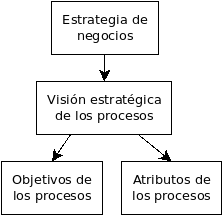
\includegraphics[width=0.3\linewidth]{marco teorico/diagramas/METO derivarivacion de objetivos} 

}

\caption{Derivación de los objetivos y atributos de los procesos}\label{fig:unnamed-chunk-8}
\end{figure}

Primero se debe tener claro el planteamiento estratégico de la
organización {[}@proce, pp. 102{]}, para ello se establece cual la
estrategia de negocio, con respecto a esto Porter identifica dos
estrategias: estrategia de menor costo, estrategia de diferenciación
{[}@nego, pp. 145{]}, para escoger una de ellas, se considerara lo
expuesto en antecedentes: situación actual mercado automóvil del
presente proyecto, y para ilustrar análisis ambiental\footnote{El
  análisis ambiental implica la vigilancia, evaluación y difusión de
  información desde los ambientes externo e interno hasta el personal
  clave de la corporación} actual se utilizara la herramienta
\textbf{matriz FODA} {[}@nego, pp. 144{]}. Se diseñara la visión
estratégica de los procesos que es una especialización de la estrategia
de negocios que entrega una expresión precisa de lo que se espera de los
procesos, lo que permitirá establecer lo siguiente:

\begin{itemize}
\tightlist
\item
  objetivos de los procesos: variables medibles de desempeño a las
  cuales se les asignan valores objetivos específicos; eliminar el
  desperdicio, eliminar la variabilidad, y dar velocidad al tiempo, se
  le asignaran valores específicos a las variables elegidas, para estos
  valores se contempla la medición del proceso actual.
\item
  Atributos de los procesos: características especificas de los
  procesos, y que cumpla con los objetivos propuestos.
\end{itemize}

\hypertarget{definir-uxe1mbito-de-proceso-a-rediseuxf1ar}{%
\subsubsection{definir ámbito de proceso a
rediseñar}\label{definir-uxe1mbito-de-proceso-a-rediseuxf1ar}}

Consiste en seleccionar y definir los procesos críticos del macroproceso
a rediseñar, a continuación se recopila información histórica de los
procesos ademas se itera y verifica el cumplimiento de los objetivos
propuestos. Se realiza entrevista al operario ejecutor del proceso
\textbf{cuestionario}, recopilada la información se decide si constituye
una unidad que debe ser mejorada.

\hypertarget{ambiente-de-ingenieruxeda-de-software}{%
\subsubsection{Ambiente de Ingeniería de
Software}\label{ambiente-de-ingenieruxeda-de-software}}

Considerando la implementación de software se establece \textbf{tipo de
desarrollo de software} entorno de desarrollo, lenguajes de programación
a utilizar, especificar tipo de servidor y base de datos.

\hypertarget{establecer-si-hacer-estudio-situaciuxf3n-actual}{%
\subsubsection{Establecer si hacer estudio situación
actual}\label{establecer-si-hacer-estudio-situaciuxf3n-actual}}

El o los procesos a mejorar son evaluado según la calidad de proceso,
con respecto al cumplimiento de los objetivos y la formalización del
proceso existente. Con esta información se decide si es no necesario
como estructura base para la elaboración de un rediseño de lo contrario
se este realizaría una reingeniería (comenzar desde cero).

\hypertarget{entender-situaciuxf3n-actual}{%
\subsection{Entender situación
actual}\label{entender-situaciuxf3n-actual}}

Se justifica esta etapa solo se en la etapa anterior se a decidido por
la realización de rediseño osea que el proceso actual es útil y por
tanto se utilizara como base para la mejora. Esta etapa se realizara con
la ayuda del jefe de taller y el operario ejecutor del proceso, del
macroproceso y proceso elegido anteriormente.

\hypertarget{modelar-la-situaciuxf3n-actual}{%
\subsubsection{Modelar la situación
actual}\label{modelar-la-situaciuxf3n-actual}}

``La ventaja de contar con un modelo formal de la situación actual es
que facilita la comunicación con quienes conocen el proceso'' {[}@proce.
pp, 114{]}. El objetivo general es entender el funcionamiento del
proceso y su coordinación con otros procesos. Se identifican actores
participantes, selecciona el patrón {[}@proce, pp. 33{]} que mas se
ajuste, se modifican las actividades según la necesidad y se establecen
elementos que intervienen en la actividad estos se clasifican en,
entrada, control, mecanismo, salida.

Para finalizar se realiza el levantamiento de proceso mediante la
elaboración de un modelo de flujo de proceso de la actividad, realizado
en Business Process Model and Notation (BPMN) basado en el libro de
Bernhard Hitpass ``BPMN Manual de Referencia y Guía
Práctica\footnote{\url{https://books.google.es/books?id=B2WyaSJD-P8C\&pg=PP5\&dq=bernhard+hitpass\&hl=es\&ei=dDcFTp_5H6S30AGdt_TxCg\&sa=X\&oi=book_result\&ct=result\#v=onepage\&q\&f=true}}''.

\hypertarget{validar-y-medir}{%
\subsubsection{Validar y medir}\label{validar-y-medir}}

Con el modelo de flujo de proceso planteado anteriormente, este es
llevado a la practica, buscando la validación del equipo cargo del
proceso de ser negativo se realizan los cambios que correspondan.
Aceptado el modelo planteado, se continua con la medición del proceso,
con el fin de cuantificar el desempeño y generar información que
posterior sera utilizada como referencia para la propuesta planteada en
el presente proyecto.

Para realizar la medición se utilizara Estudios de tiempos para poder
establecer un estándar trabajo, en colaboración con el operador se mide
el tiempo necesario para la realización del proceso completo {[}@heizer,
pp. 413{]}. Para este caso practico por ejemplo en el proceso de gestión
de inventario se propone el uso de KPI (Key Performance Indicator) que
contemple el rendimiento de ubicación correcta del producto, la formula
postula que:

\begin{center}
$Ubicacióncorrecta = \frac{Despacho}{Despacho-Error en ubicación}$
\end{center}

El establecer calificaciones para este indicador, permitirá medir el
movimiento innecesario del operario en al pickear un producto.

\hypertarget{rediseuxf1o}{%
\subsection{Rediseño}\label{rediseuxf1o}}

Para esta etapa se contempla la filosofía de lean manufacturing, por lo
que se implementara 5's debido a que se dice si en una empresa no ha
funcionado la implementación de las 5's, cualquier otro sistema de
mejoramiento de procesos esta destinado a fracasar {[}@leanmanu, pp.
147{]}. Se realiza en colaboración de jefe de taller y el operario
ejecutor del proceso.

\hypertarget{establecer-direcciuxf3n-del-cambio}{%
\subsubsection{Establecer dirección del
cambio}\label{establecer-direcciuxf3n-del-cambio}}

Se establecerán un conjunto de diferencias entre el actual proceso y la
propuesta para generar cambios reales necesarios según objetivos, para
identificar las fallas del actual proceso se empleara la herramienta de
AMEF {[}@leanmanu, pp. 223{]} con el objetivo construir información útil
para el rediseño. Identificar la dirección del cambio si es horizontal,
vertical, interno o externo. Como primicia los actores no deberían
diferir de los ya indicados, por el contrario se puede inferir en la
adición de nuevas tareas.

\hypertarget{seleccionar-tecnologuxedas-habilitantes}{%
\subsubsection{Seleccionar tecnologías
habilitantes}\label{seleccionar-tecnologuxedas-habilitantes}}

Consiste en buscar y evaluar las tecnologías existentes y que hacen
factible el cambio propuesto. Como primicia en esta etapa el autor
propone construir un software basado en lenguajes Open Source y Free
Source, con el objetivo de ajustar el software a las necesidades del
proceso. Otro aspecto importante del software es la nula inversión. El
software sera diseñado como aplicativo web basado en WMS, por lo tanto
sera necesario el uso de un buscador, razón de adoptar este diseño es su
compatibilidad con diferentes dispositivos.

El hardware a utilizar sera el computador existente en el área almacén,
este también sera utilizado como servidor local por ende tampoco
presenta un costo. Se destaca que se podrá acceder desde dispositivos
móviles (smartphones), siempre que estén conectados a la misma red que
el servidor (computador área almacén). Se agrega un también un lector de
barras con conexión USB, el cual también puede ser conectado a
dispositivos móviles mediante un adaptador OTG.

\hypertarget{modelar-evaluar-rediseuxf1o}{%
\subsubsection{Modelar evaluar
rediseño}\label{modelar-evaluar-rediseuxf1o}}

En general consiste en analizar la información de fallas, e integrar
nuevas tareas al o los procesos propuestos, se considera utilizar apoyo
tecnológicos básico, en colaboración del operador se realiza el proceso
completo, a continuación se evalúa el desempeño del proceso con respecto
al cumplimiento de objetivos, de haber fallos se reparan. Se realiza el
levantamiento de proceso al igual que el levantamiento del proceso
actual (BPMN).

\hypertarget{detallar-y-probar-rediseuxf1o}{%
\subsubsection{Detallar y probar
rediseño}\label{detallar-y-probar-rediseuxf1o}}

Se detalla el funcionamiento del proceso en conjunto al software.

\begin{itemize}
\tightlist
\item
  Detalle de procedimiento: se establece en detalle responsabilidades,
  especificación de situaciones{[}@proce, pp. 162{]} y se complementara
  con la elaboración de manual de las distintas tareas del proceso.
\item
  Detalle apoyo computacional

  \begin{itemize}
  \tightlist
  \item
    Rutinas automatizadas: Las rutinas a implementar se detallaran para
    poder ser programadas, se contemplan el uso de modelos de análisis
    lógicos, predictivos.
  \item
    Apoyo información: Se especifica la información a entregar a las
    diferentes actividades del proceso, como también la forma en que se
    entregara.
  \end{itemize}
\item
  Prueba: Se realizan pruebas pilotos del rediseño propuesto
  involucrando, un prototipo del software propuesto, se evalúan los
  resultados.
\end{itemize}

\hypertarget{implementar}{%
\subsection{Implementar}\label{implementar}}

\hypertarget{construir-software}{%
\subsubsection{Construir software}\label{construir-software}}

\hypertarget{implementar-software}{%
\subsubsection{implementar software}\label{implementar-software}}

\hypertarget{implementar-procesos}{%
\subsubsection{Implementar procesos}\label{implementar-procesos}}

\hypertarget{resultados-esperados}{%
\section{Resultados Esperados}\label{resultados-esperados}}

\newpage

\hypertarget{capuxedtulo-iv-desarrollo}{%
\section{Capítulo IV: Desarrollo}\label{capuxedtulo-iv-desarrollo}}

\hypertarget{definir-proyecto-1}{%
\subsection{Definir proyecto}\label{definir-proyecto-1}}

\hypertarget{establecer-objetivo-del-rediseuxf1o-1}{%
\subsubsection{Establecer objetivo del
rediseño}\label{establecer-objetivo-del-rediseuxf1o-1}}

\hypertarget{definir-uxe1mbito-de-proceso-a-rediseuxf1a}{%
\subsubsection{Definir ámbito de proceso a
rediseña}\label{definir-uxe1mbito-de-proceso-a-rediseuxf1a}}

\hypertarget{ambiente-de-ingenieruxeda-de-software-segun-figuero-romero}{%
\subsubsection{Ambiente de Ingeniería de Software (segun figuero
romero)}\label{ambiente-de-ingenieruxeda-de-software-segun-figuero-romero}}

\hypertarget{establecer-si-hacer-estudio-situaciuxf3n-actual-1}{%
\subsubsection{Establecer si hacer estudio situación
actual}\label{establecer-si-hacer-estudio-situaciuxf3n-actual-1}}

\hypertarget{analisis-de-la-situcion-actual}{%
\subsection{Analisis de la situcion
actual}\label{analisis-de-la-situcion-actual}}

\hypertarget{inventarios}{%
\subsubsection{Inventarios}\label{inventarios}}

\hypertarget{tipo-de-producto-ica-6363}{%
\paragraph{tipo de producto ICA 6363}\label{tipo-de-producto-ica-6363}}

\hypertarget{analisis-de-niveles-de-inventario}{%
\paragraph{Analisis de niveles de
inventario}\label{analisis-de-niveles-de-inventario}}

\textbf{Arreglar porcentaje}

\hypertarget{analisis-abc-de-inventarios}{%
\paragraph{Analisis ABC de
inventarios}\label{analisis-abc-de-inventarios}}

MODELOS DE INVENTARIO

Costos de mantener, ordenar y preparar inventario

levanta, diagnosti, control

\hypertarget{demanda}{%
\subsubsection{Demanda}\label{demanda}}

\hypertarget{recepciuxf3n}{%
\subsubsection{Recepción}\label{recepciuxf3n}}

\hypertarget{proceso}{%
\paragraph{Proceso}\label{proceso}}

La recepción es una etapa primordial debido a que la eliminación de
errores al momento de ingresar repuestos al inventario, condiciona el
despacho a incurrir en un error (descartando movimiento de inventario
entre recepción y despacho). el proceso actual carece de un sistema
tecnológico de información por tanto es propenso a la generación de
errores. La figura @ref(fig:bpmnin) muestra de el flujo de proceso de
recepeción

\begin{figure}[H]

{\centering 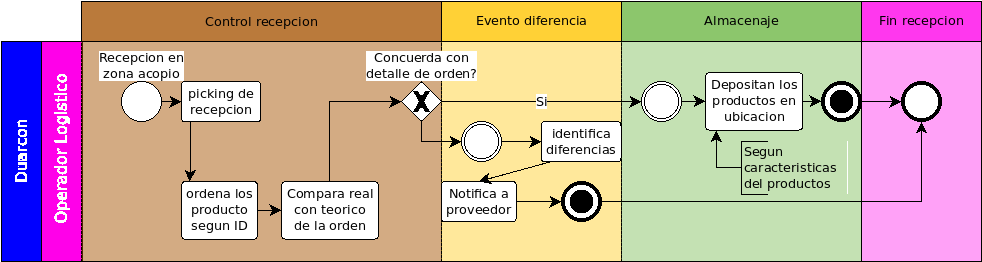
\includegraphics[width=0.5\linewidth]{marco teorico/Almacenaje} 

}

\caption{BPMN proceso recepción}\label{fig:unnamed-chunk-9}
\end{figure}

\hypertarget{costo}{%
\paragraph{Costo}\label{costo}}

El análisis de facturas de compra permite el análisis de costos
asociados a recepción, se considera el numero de compras al mes y el
monto a pagar también es importante el proveedor debido a que en el
inventario existente se mantiene productos de solo 2 proveedores
(Autotec, Ital frenos), la figura @ref(table: mayores numeros de
recepcion)

Con esta información se puede realizar un análisis del costo de orden
con respecto a las compras en sucursal del distribuidor, el costo se
considera monetario como también tiempo utilizado del operador logístico
que incurre en su ausencia del almacén, la figura @ref(fig:camino)
muestra la distancia que debe recorrer el operador para adquirir
repuestos.

\begin{figure}[H]

{\centering \includegraphics[width=1\linewidth]{marco teorico/image/caminoabaste} 

}

\caption{Trayecto para adquirir repuestos}\label{fig:unnamed-chunk-11}
\end{figure}

Para adquirir repuestos, el operador debe ir a la Av. 10 de Julio
Huamachuco, en donde se encuentran los principales distribuidores de
repuestos, la distancia recorrer es de 34 km ida y vuelta para realizar
esta operación el operador indica que toma entre 90 min a 2 horas
aproximadamente dependiendo del trafico. Otro costo asociado es el costo
de bencina, el vehículo utilizado es un wolkswagen 32321 la tabla
@ref(fig:caractrans) presenta las características del vehículo. Otro
costo a considerar es el uso de la autopista, este costo se presenta
cada vez que el vehículo atraviesa el pórtico de la autopista.

\begin{figure}[H]

{\centering \includegraphics[width=0.2\linewidth]{marco teorico/image/caminoabaste} 

}

\caption{Caracteristicas del vehiculo de transporte}\label{fig:unnamed-chunk-12}
\end{figure}

\begin{figure}
\centering
\includegraphics{fig/caminoabaste.png}
\caption{caminoabaste}
\end{figure}

Con la presente información se puede realizar estimar los costos
asociado a orden de producto

El costo de orden (\textbf{suma el costo de ir a comprar, count date})
del stock que se mantiene en el almacén corresponde \textbf{su} en
constraste a \textbf{q prod no almacen} desde \textbf{la fecha recep}
según los libros de recepción, recepcion producto de los proveedores
marcados en la tabla

\textbf{compara repuesto bodega con los iCA}

\hypertarget{despacho}{%
\subsubsection{Despacho}\label{despacho}}

\begin{figure}[H]

{\centering 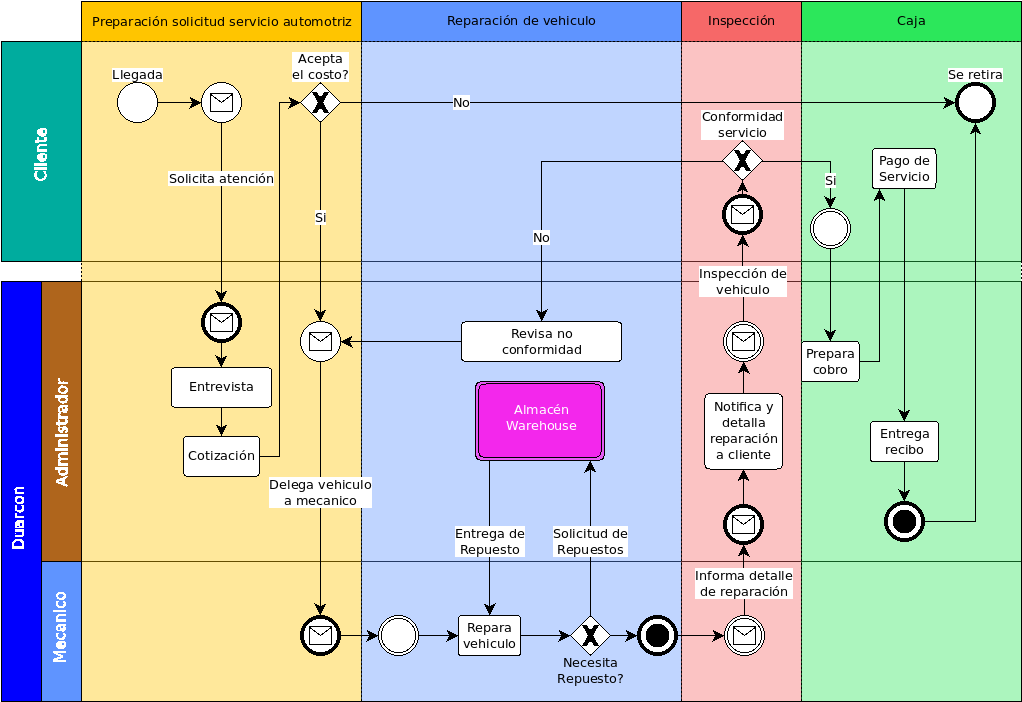
\includegraphics[width=0.5\linewidth]{marco teorico/D_servicio} 

}

\caption{BPMN de servicio reparación}\label{fig:unnamed-chunk-13}
\end{figure}

tiempo error

\hypertarget{redisenar}{%
\subsection{Redisenar}\label{redisenar}}

\hypertarget{preparacion-de-almacen}{%
\subsubsection{Preparacion de almacen}\label{preparacion-de-almacen}}

\hypertarget{implementar-5s}{%
\paragraph{Implementar 5's}\label{implementar-5s}}

\hypertarget{section}{%
\paragraph{}\label{section}}

\hypertarget{ubicaciones}{%
\paragraph{Ubicaciones}\label{ubicaciones}}

Para identificar las distintas posiciones que tendrá el stock, se
implementara una clasificación que según sector (véase figura
@ref(fig:layoutinvnt)), columna y fila

\begin{figure}[H]

{\centering 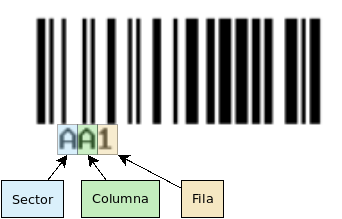
\includegraphics[width=0.5\linewidth]{marco teorico/image/barEstruc} 

}

\caption{Intrepretación codigo de barras ubicacion}\label{fig:unnamed-chunk-14}
\end{figure}

ADMINISTRACIÓN DE INVENTARIOS Conteo cíclico MODELOS DE INVENTARIO PARA
DEMANDA INDEPENDIENTE Modelo de la cantidad económica a ordenar (EOQ) 2.
Modelo de la cantidad económica a producir 3. Modelo de descuentos por
cantidad MODELOS PROBABILÍSTICOS E INVENTARIO DE SEGURIDAD

\hypertarget{control-mediante-kpi}{%
\subsubsection{Control mediante KPI}\label{control-mediante-kpi}}

\hypertarget{estudios-de-tiempo}{%
\paragraph{Estudios de tiempo}\label{estudios-de-tiempo}}

\hypertarget{hardware}{%
\subsubsection{Hardware}\label{hardware}}

\hypertarget{computador}{%
\paragraph{Computador}\label{computador}}

\hypertarget{lector-barras}{%
\paragraph{Lector barras}\label{lector-barras}}

Para garantizar velocidad en el ingreso de información se utilizara un
lector de barras, este se prevee su uso en la lectura de código de los
productos y en la lectura de ubicación.

\begin{figure}[H]

{\centering 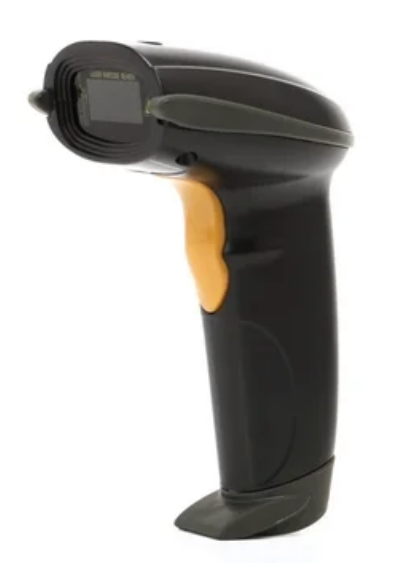
\includegraphics[width=0.2\linewidth]{marco teorico/image/lectorbar} 

}

\caption{Lector de barras}\label{fig:unnamed-chunk-15}
\end{figure}

\hypertarget{software}{%
\subsubsection{Software}\label{software}}

\hypertarget{software-prototipos}{%
\paragraph{Software prototipos}\label{software-prototipos}}

Para realizar pruebas con el prototipo de software se utilizara el
gestor de base de datos \textbf{phpMyAdmin}, se construirá una
estructura relacional tal como muestra la figura @ref(fig:bdest) Se
construlle la estructura básica de la base de datos * MariaDB

\begin{figure}[H]

{\centering 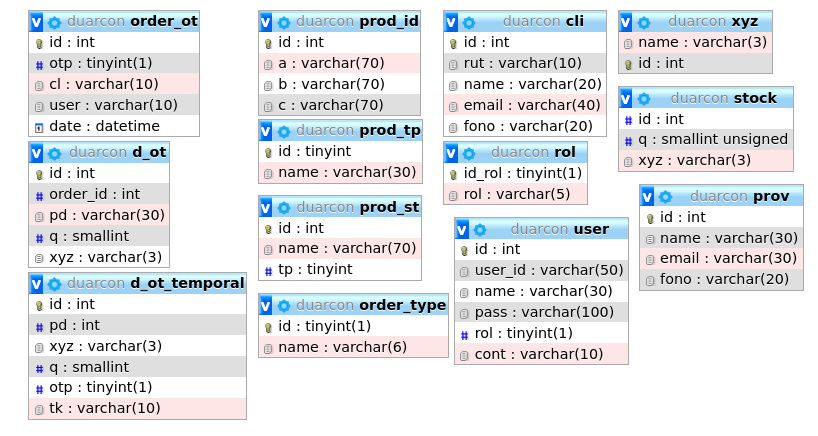
\includegraphics[width=1\linewidth]{marco teorico/Screenshot from 2021-11-01 20-35-27} 

}

\caption{Estructura base de datos relacional}\label{fig:unnamed-chunk-16}
\end{figure}

\hypertarget{direcciones-de-cambio}{%
\subsubsection{Direcciones de cambio}\label{direcciones-de-cambio}}

\hypertarget{tecnologuxedas-habilitantes}{%
\subsubsection{Tecnologías
Habilitantes}\label{tecnologuxedas-habilitantes}}

\hypertarget{modelamiento-del-rediseuxf1o}{%
\subsubsection{Modelamiento del
Rediseño}\label{modelamiento-del-rediseuxf1o}}

\hypertarget{rediseuxf1o-subproceso-entrada-de-productos}{%
\paragraph{Rediseño Subproceso Entrada de
productos}\label{rediseuxf1o-subproceso-entrada-de-productos}}

\hypertarget{rediseuxf1o-subproceso-despacho-de-productos}{%
\paragraph{Rediseño Subproceso Despacho de
productos}\label{rediseuxf1o-subproceso-despacho-de-productos}}

\hypertarget{indicadores-de-desempeuxf1o-loguxedstico}{%
\paragraph{Indicadores de desempeño
logístico}\label{indicadores-de-desempeuxf1o-loguxedstico}}

kpi estudio de tiempo \#\#\#\# Rediseño manejo multibodega: Interacción
con bodega externa

\hypertarget{implementar-1}{%
\subsection{Implementar}\label{implementar-1}}

\hypertarget{construir-software-1}{%
\subsubsection{Construir software}\label{construir-software-1}}

\hypertarget{implementar-software-1}{%
\subsubsection{Implementar software}\label{implementar-software-1}}

\hypertarget{implementar-procesos-1}{%
\subsubsection{Implementar procesos}\label{implementar-procesos-1}}

\hypertarget{definir-proyecto-2}{%
\subsection{Definir proyecto}\label{definir-proyecto-2}}

\hypertarget{entender-situacion-actual}{%
\subsection{Entender situacion actual}\label{entender-situacion-actual}}

\hypertarget{analisis-de-niveles-de-inventario-1}{%
\subsubsection{Analisis de niveles de
inventario}\label{analisis-de-niveles-de-inventario-1}}

\hypertarget{analisis-abc-de-inventarios-1}{%
\subsubsection{Analisis ABC de
inventarios}\label{analisis-abc-de-inventarios-1}}

\hypertarget{rediseno}{%
\subsection{Rediseno}\label{rediseno}}

\hypertarget{procedimiento-para-la-gestiuxf3n-de-inventarios}{%
\subsubsection{Procedimiento para la gestión de
inventarios}\label{procedimiento-para-la-gestiuxf3n-de-inventarios}}

\hypertarget{capuxedtulo-v-evaluaciuxf3n-econuxf3mica}{%
\section{Capítulo V: EVALUACIÓN
ECONÓMICA}\label{capuxedtulo-v-evaluaciuxf3n-econuxf3mica}}

\hypertarget{factibilidad}{%
\subsection{Factibilidad}\label{factibilidad}}

\hypertarget{factibilidad-tuxe9cnica}{%
\subsubsection{Factibilidad técnica}\label{factibilidad-tuxe9cnica}}

\hypertarget{factibilidad-operativa}{%
\subsubsection{Factibilidad operativa}\label{factibilidad-operativa}}

\hypertarget{beneficios-tangibles}{%
\subsection{Beneficios Tangibles}\label{beneficios-tangibles}}

\hypertarget{beneficios-intangibles}{%
\subsection{Beneficios Intangibles:}\label{beneficios-intangibles}}

\hypertarget{costos}{%
\subsection{Costos:}\label{costos}}

\hypertarget{cuxe1lculo-del-van}{%
\subsubsection{Cálculo del VAN}\label{cuxe1lculo-del-van}}

\hypertarget{conclusiuxf3n-de-la-factibilidad}{%
\subsection{Conclusión de la
factibilidad}\label{conclusiuxf3n-de-la-factibilidad}}

\hypertarget{capuxedtulo-iv-presentaciuxf3n-resultados}{%
\section{Capítulo IV: PRESENTACIÓN
RESULTADOS}\label{capuxedtulo-iv-presentaciuxf3n-resultados}}

\hypertarget{procesamiento-de-los-datos.}{%
\subsection{Procesamiento de los
datos.}\label{procesamiento-de-los-datos.}}

\hypertarget{resultados}{%
\subsection{Resultados}\label{resultados}}

\hypertarget{capuxedtulo-v-conclusiones}{%
\section{Capítulo V: CONCLUSIONES}\label{capuxedtulo-v-conclusiones}}

\hypertarget{discusiuxf3n}{%
\subsection{Discusión}\label{discusiuxf3n}}

\begin{figure}

{\centering 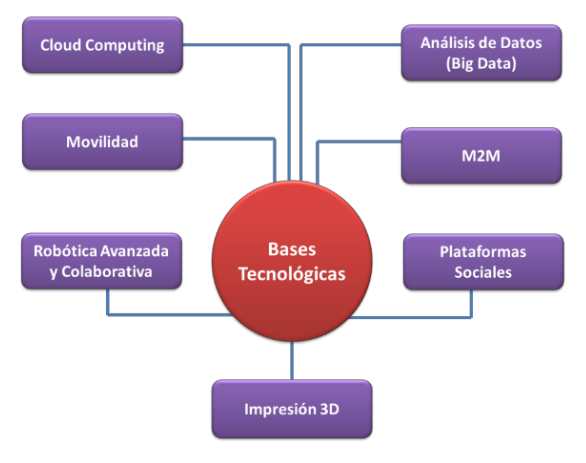
\includegraphics[width=0.5\linewidth]{marco teorico/Screenshot from 2021-11-01 14-03-25} 

}

\caption{Tecnologías Básicas en que se sustenta la industria 4.0}\label{fig:unnamed-chunk-17}
\end{figure}

\begin{figure}

{\centering 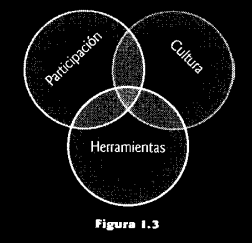
\includegraphics[width=0.5\linewidth]{marco teorico/Screenshot from 2021-11-02 17-24-54} 

}

\caption{Implicacion al éxito}\label{fig:unnamed-chunk-18}
\end{figure}

estrategia de diferenciación \#\# Referencia

\end{document}
